\section{Qualidade do Código Fonte}

\subsection{SonarQube}

\begin{figure}[H]

  \centering

  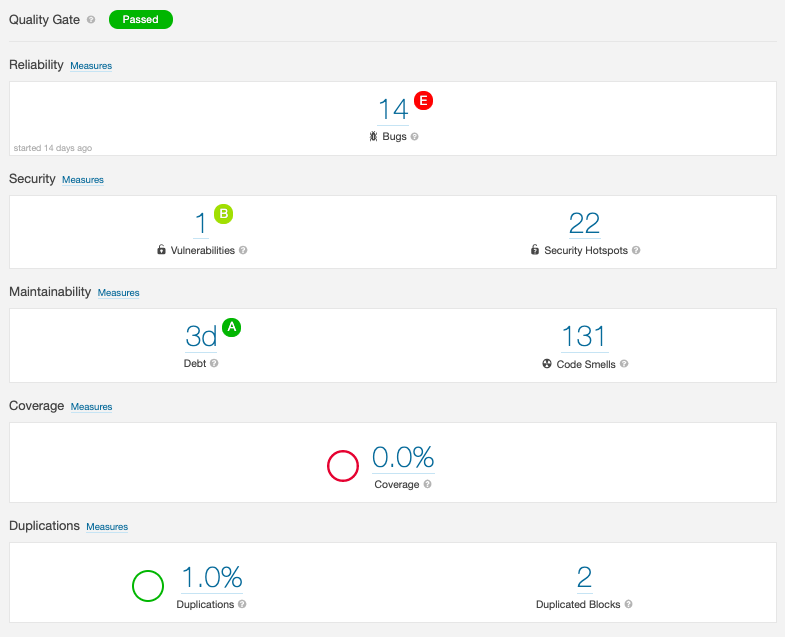
\includegraphics[scale = 0.5]{sonarEvaluation.png}

  \caption {Menu geral de avaliação do SonarQube}

  \label {fig01}

\end{figure}


\par Como se pode ver pela figura~\ref{fig:fig01} este projeto possui alguns bugs, pelo menos 1 vulnerabilidade uma quantidade consideravel de code smells e 2 blocos duplicados.


De seguida apresenta-se um relatório detalhado dos tipos de erros e da sua gravidade:
\subsection{Bugs}
versão com bugs, sem bugs, com smells sem smells (por tipos de smells) -> descriminar o impacto dos smells
\subsubsection{Blocker Bugs:}
\begin{itemize}
\item Não usar blocos try/catch ao escrever em ficheiros.\newline


\par Podemos visualizar nas seguintes imagens o código analisado e a solução respetiva.

\begin{figure}[H]

  \centering

  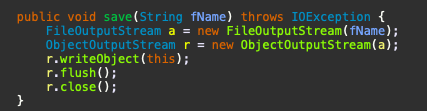
\includegraphics[scale = 0.5]{preWriteTryCatch.png}

  \caption {Código com bug}

  \label {fig02}

\end{figure}

\begin{figure}[H]

  \centering

  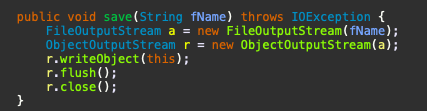
\includegraphics[scale = 0.5]{posWriteTryCatch.png}

  \caption {Código corrigido}

  \label {fig03}

\end{figure}

\item Não usar blocos try/catch ao ler de ficheiros.\newline


\par Podemos visualizar nas seguintes imagens o código analisado e a solução respetiva.


\begin{figure}[H]

  \centering

  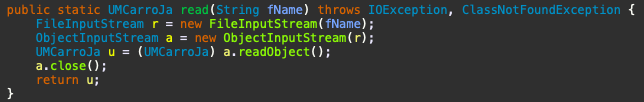
\includegraphics[scale = 0.5]{preReadTryCatch.png}

  \caption {Código com bug}

  \label {fig04}

\end{figure}

\begin{figure}[H]

  \centering

  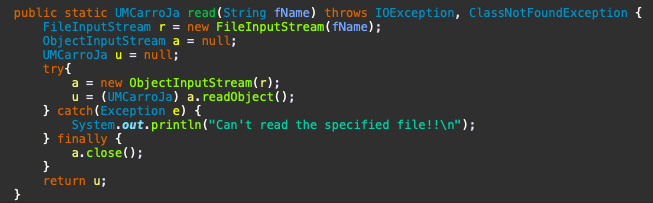
\includegraphics[scale = 0.5]{posReadTryCatch.png}

  \caption {Código corrigido}

  \label {fig05}

\end{figure}

\end{itemize}

\subsubsection{Critical Bugs:}
\begin{itemize}
\item Guardar e reutilizar variáveis random. \newline


\par Para resolver o problema basta verificar que o random estava a ser gerado sempre que a função \textit{getTraficDelay()} era invocada. Para resolver basta gerar o random uma unica vez quando a classe for criada e usar o mesmo sempre que a função em causa for invocada.

\begin{figure}[H]

  \centering

  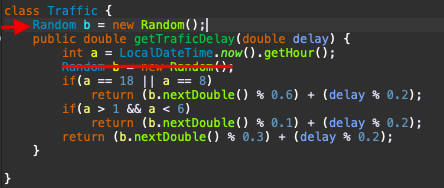
\includegraphics[scale = 0.5]{randomGeneration.png}

  \caption {Recolocação do método de geração de um número Random}

  \label {fig06}

\end{figure}
\end{itemize}

\subsubsection{Major Bugs:}
\begin{itemize}
\item Não obrigar a usar o método redifinido usando override.\newline


.................Rever...............
\par Para resolver este problema fo preciso renomear o método equals para o método isEqual, visto que usando um \textit{@Override} este método obrigaria a implementar um método de super tipo.

\begin{figure}[H]

  \centering

  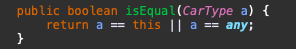
\includegraphics[scale = 0.5]{isEqualFunction.png}

  \caption {Definição da função isEqual}

  \label {fig07}

\end{figure}

\end{itemize}

\subsubsection{Minor Bugs:}
\begin{itemize}
\item Obrigar o override do equals e não o do método hashCode().\newline


\par Para corrigir este problema, basta definir um hashCode() que chame super.hashCode() como se pode ver na figura seguinte.

\begin{figure}[H]

  \centering

  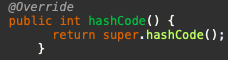
\includegraphics[scale = 0.6]{hashCode.png}

  \caption {Solução do problema de Override do método hashCode}

  \label {fig08}

\end{figure}

\end{itemize}


\subsection{Vulnerabilitys}
\begin{itemize}
\item Utilizar printStackTrace() pode revelar informação sensivel.\newline
\end{itemize}

\subsection{CodeSmells}

\begin{itemize}
\item Blocos de código repetidos.\newline
\end{itemize}





